\documentclass[14pt,aspectratio=1610]{beamer}

\usepackage[brazil]{babel}
\usepackage[utf8]{inputenc}
%\UseRawInputEncoding
\usepackage[T1]{fontenc}
\usepackage{Sweave}
\usepackage{animate}
\usepackage{amsbsy}
\usepackage{amsfonts}
\usepackage{amsmath}
\usepackage{amssymb}
\usepackage{amsthm}
\usepackage[toc,page,title,titletoc]{appendix}
\usepackage[fixlanguage]{babelbib}
%\usepackage[pdftex]{color}
\usepackage{dsfont}
\usepackage{esvect}
\usepackage[labelfont=bf]{caption}
\usepackage{float}
\usepackage[Glenn]{fncychap}%Sonny %Conny %Lenny %Glenn %Renje %Bjarne %Bjornstrup
%\usepackage{geometry, calc, color, setspace}%
%\geometry{a4paper, headsep=1.0cm, footskip=1cm, lmargin=3cm, rmargin=2cm, tmargin=3cm, bmargin=2cm}
\usepackage{graphicx}
\usepackage{indentfirst}%Para indentar os parágrafos automáticamente
\usepackage{lipsum}
\usepackage{longtable}
\usepackage{mathtools}
\usepackage{listings}%Inserir codigo do R no latex
\usepackage{multirow}
\usepackage{multicol}
\usepackage{natbib}
\bibliographystyle{abbrvnat3}
\usepackage[figuresright]{rotating}
\usepackage{spalign}
%\usepackage{pgfpages}
\usepackage{pgfplots}
\usepackage{tikz}
\usepackage{color, colortbl}
\usepackage{ragged2e}%para justificar o texto dentro de algum ambiente
\definecolor{Gray}{gray}{0.9}
\definecolor{LightCyan}{rgb}{0.88,1,1}


\usepackage[all]{xy}
\usepackage{hyperref,bookmark}
\hypersetup{
  colorlinks=true,
  linkcolor=blue,
  citecolor=red,
  filecolor=blue,
  urlcolor=blue,
}

\usetheme{boxes}
%\usecolortheme[RGB={193,0,0}]{structure}

%\setbeamertemplate{footline}[frame number]
%\setbeamertemplate{footline}[text line]{%
%  \parbox{\linewidth}{\vspace*{-8pt}\hfill\date{}\hfill\insertshortauthor\hfill\insertpagenumber}}
\beamertemplatenavigationsymbolsempty
\renewcommand{\vec}[1]{\mbox{\boldmath$#1$}}
\newtheorem{Teorema}{Teorema}
\newtheorem{Proposicao}{Proposição}
\newtheorem{Definicao}{Definição}
\newtheorem{Corolario}{Corolário}
\newtheorem{Demonstracao}{Demonstração}
\newcommand{\bx}{\ensuremath{\bar{x}}}
\newcommand{\Ho}{\ensuremath{H_{0}}}
\newcommand{\Hi}{\ensuremath{H_{1}}}


\apptocmd{\frame}{}{\justifying}{} % Allow optional arguments after frame.

\title{MAF 261 - Estatística Experimental}
\author{Prof. Fernando de Souza Bastos}
\institute{Instituto de Ciências Exatas e Tecnológicas\texorpdfstring{\\ Universidade Federal de Viçosa}{}\texorpdfstring{\\ Campus UFV - Florestal}{}}
\date{2018}
\newcommand\mytext{Aula 9}
\newcommand\mytextt{Fernando de Souza Bastos}
\makeatletter
\setbeamertemplate{footline}
{
  \leavevmode%
  \hbox{%
  \begin{beamercolorbox}[wd=.333333\paperwidth,ht=2.25ex,dp=1ex,center]{author in head/foot}%
    \usebeamerfont{author in head/foot}\mytext
  \end{beamercolorbox}%
  \begin{beamercolorbox}[wd=.333333\paperwidth,ht=2.25ex,dp=1ex,center]{title in head/foot}%
    \usebeamerfont{title in head/foot}\mytextt
  \end{beamercolorbox}%
  \begin{beamercolorbox}[wd=.333333\paperwidth,ht=2.25ex,dp=1ex,right]{date in head/foot}%
    \usebeamerfont{date in head/foot}\insertshortdate{}\hspace*{2em}
    \insertframenumber{} / \inserttotalframenumber\hspace*{2ex} 
  \end{beamercolorbox}}%
  \vskip0pt%
}
\makeatother


\providecommand{\arcsin}{} \renewcommand{\arcsin}{\hspace{2pt}\textrm{arcsen}}
\providecommand{\sin}{} \renewcommand{\sin}{\hspace{2pt}\textrm{sen}}
%\newtheorem{Teorema}{Teorema}
%\newtheorem{Proposicao}{Proposição}
%\newtheorem{Definicao}{Definição}
%\newtheorem{Corolario}{Corolário}
%\newtheorem{Demonstracao}{Demonstração}

% Layout da pagina
\hypersetup{pdfpagelayout=SinglePage}
\begin{document}
\Sconcordance{concordance:Aula16.tex:Aula16.Rnw:%
1 216 1}


\frame{\titlepage}

\begin{frame}{}
\frametitle{\bf Sumário}
\tableofcontents
\end{frame}

\section{Esquema em Parcelas Subdivididas}
\begin{frame}{}
\frametitle{Introdução}
\begin{block}{}
\justifying



\end{block}
\end{frame}

\begin{frame}{}
\frametitle{}
\begin{block}{}
\begin{figure}[H]
     \centering
\pgfdeclareimage[height=8cm,width=13cm]{fig1}{Figuras/Fig1}
\pgfuseimage{fig1}
\end{figure}
\end{block}
\end{frame}

\begin{frame}{}
\frametitle{}
\begin{block}{}
\begin{figure}[H]
     \centering
\pgfdeclareimage[height=8cm,width=13cm]{fig1}{Figuras/Fig7}
\pgfuseimage{fig1}
\end{figure}
\end{block}
\end{frame}

% \begin{frame}{}
% \frametitle{}
% \begin{block}{}
% 
% 
% \begin{columns}
%         \column{7cm}
% \justifying
% {\bf Croqui de um Experimento:} É o plano formal para conduzir o experimento. Inclui a escolha dos fatores, níveis, tratamentos e números de réplicas. Também pode ser entendido como a maneira como os tratamentos são designados às unidades experimentais.
% 
%         \column{6cm}
%  \begin{block}{}
% 
% \pgfdeclareimage[height=5cm,width=6cm]{fig1}{Figuras/Fig1}
% \pgfuseimage{fig1}
% \end{block}
% \end{columns}
% \end{block}
% \end{frame}

% \begin{frame}{}
% \frametitle{}
% \begin{block}{}
% \justifying
% Modelo geral de um processo para o delineamento de experimentos:
% \begin{figure}[H]
%     \centering
%     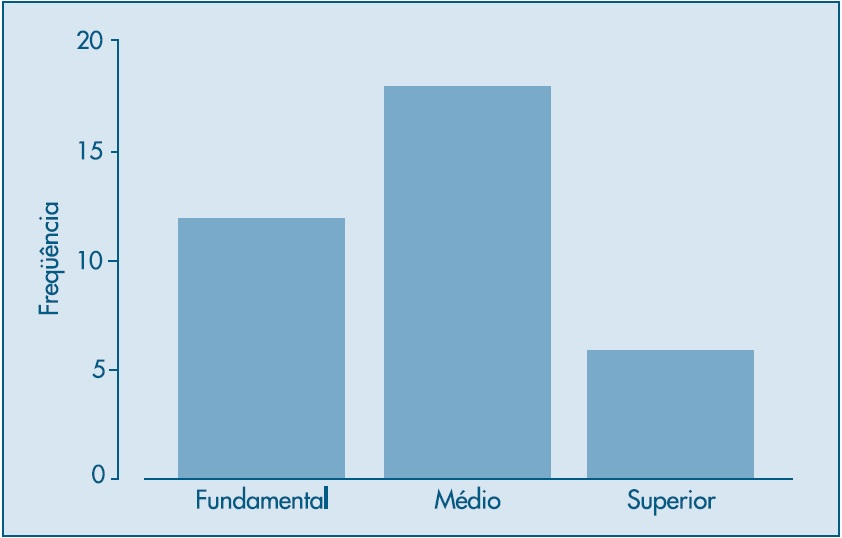
\includegraphics[scale=0.5]{Figuras/Fig3.gif}
%     %\caption{}
%     %\label{figRotulo}
%   \end{figure}
% \end{block}
% \end{frame}

\begin{frame}{}
\frametitle{}
\begin{block}{}
\begin{figure}[H]
    \centering
    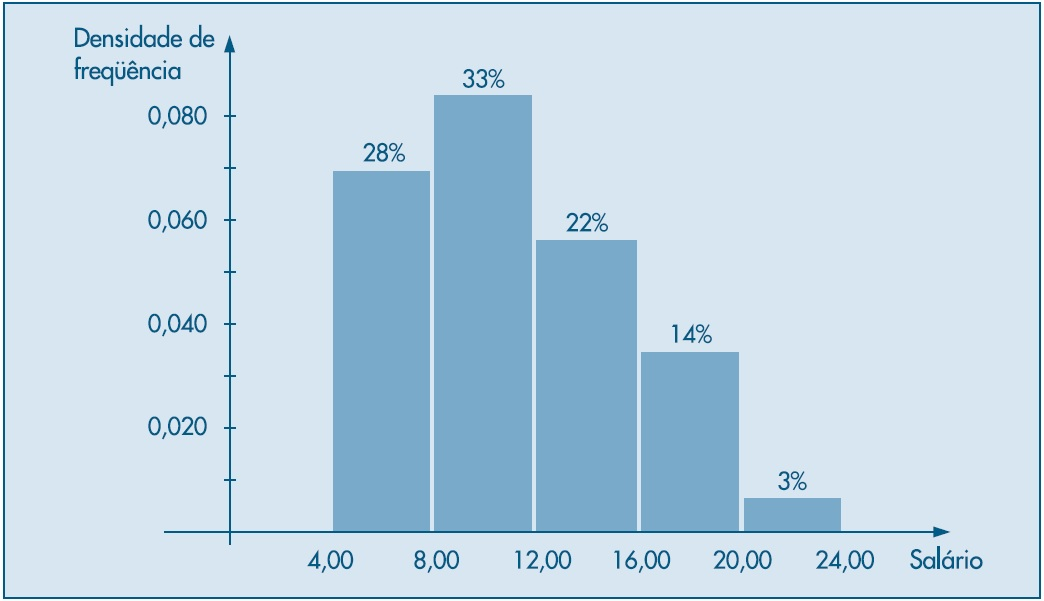
\includegraphics[scale=0.5]{Figuras/Fig5}
    %\caption{}
    %\label{figRotulo}
  \end{figure}
\end{block}
\end{frame}

\begin{frame}{}
\frametitle{}
\begin{block}{}
\begin{figure}[H]
    \centering
    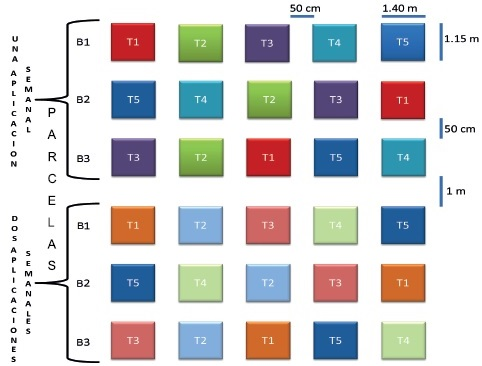
\includegraphics[scale=0.3]{Figuras/Fig6}
    %\caption{}
    %\label{figRotulo}
  \end{figure}
\end{block}
\end{frame}

\begin{frame}[allowframebreaks]
\frametitle{Referências Bibliográficas}
\bibliography{bibliografia}
\end{frame}

\end{document}
